\section{Cloud Based Processing, Storage and Inference}
The following sections of the report discuss implementations involving Cloud-Based services, i.e. Lambda, Sagemaker, S3, and API Gateway to name a few.
%Anurag's stuff
\subsection{Telemetry Pipeline 1/3 - Triggering Lambda}
One of the three pipelines, involves the transportation of wireless telemetry data directly to the Cloud via the usage of API Gateway and triggering Lambda services. 
\subsubsection{API Gateway Setup to S3 Remote Upload}
The first part to the pipeline to the cloud is the entry into the AWS Cloud. While the possiblity exists to upload directly to S3 via usage of the AWS Command Line Interface (CLI), this is not the preferred way as usage of the Cloud Service cannot be easily monitored and there exists too much control of configurations via the AWS CLI that could be exploited. It is preferred to limit as much access as required to the Cloud from the remote location, primarily for security reasons and for ease of use as well. 

The API Gateway follows the method and resource plan as per the design in Figure \ref{fig:api_gateway_methods}, which described which methods (e.g. POST, GET, PUT, etc...) can be applied to various resources (e.g. .../{s3-bucket}/). To implement the design after setting up the API Gateway, a resource is attached to the address as per Figure \ref{fig:attach_new_resource_api_gateway}. This resource can then be given a name either under \textit{/s3} or further into the s3 address as \textit{/s3/\{bucket\}}.

\begin{figure}[ht]
    \centering
    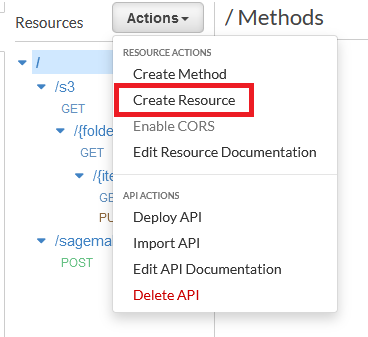
\includegraphics{pages/Chapter4/Chapter 4 Images/create_method_api_gateway.png}
    \caption{Creating a new resource}
    \label{fig:attach_new_resource_api_gateway}
\end{figure}

Once the resource is created and an appropriate name given, then a method can be attached to it. Generally a GET method will be used to retrieve data from the S3 bucket or it can also be used to get a list of all items within the S3 bucket. A PUT method will allow the upload of a unique data object just one time to the S3 Bucket, whereas a POST will allow repeated uploads of the same unique data object. 

The method can be attached to a resource as seen in Figure \ref{fig:attach_new_resource_api_gateway} but instead \textit{Create Method} must be selected. Then from the method execution dashboard in Figure \ref{fig:api_gateway_integration_req}, the integration request options should be selected and a setup similar to the options shown in Figure \ref{fig:integration_request_settings} should be chosen. This will forward the GET request to the S3 endpoint and retrieve the data item or list of items as required.

\begin{figure}[ht]
    \centering
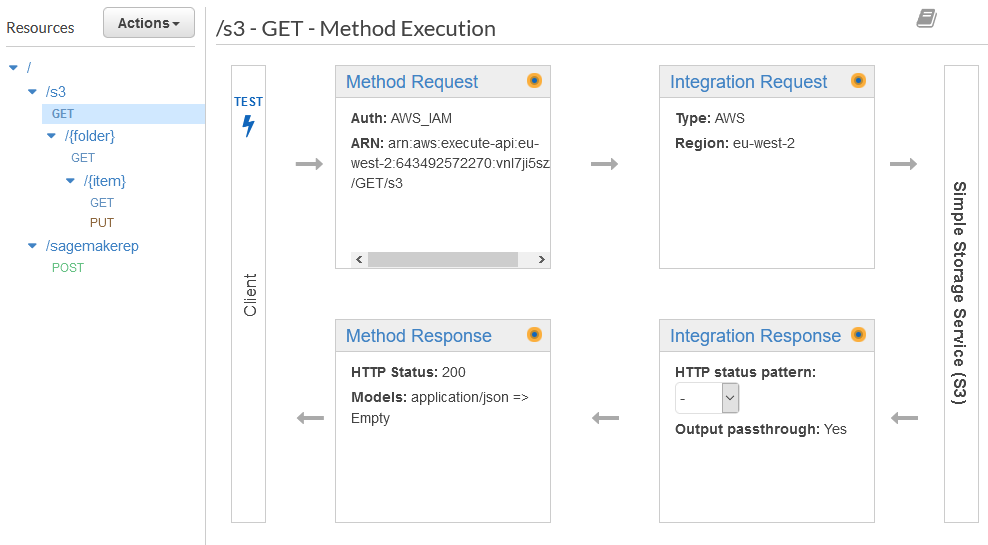
\includegraphics[width=1\linewidth]{pages/Chapter4/Chapter 4 Images/get_method_execution_1.png}
    \caption{Method Execution Dashboard, where settings for security, and redirecting and response settings can be setup}
    \label{fig:api_gateway_integration_req}
\end{figure}

\begin{figure}[ht]
    \centering
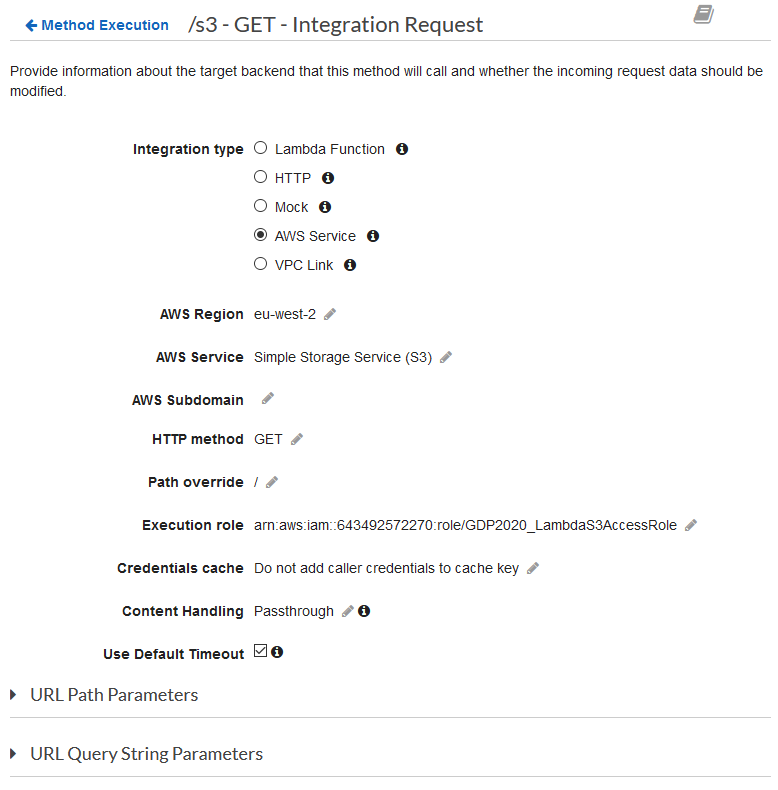
\includegraphics[width=1\linewidth]{pages/Chapter4/Chapter 4 Images/get_method_execution_2.png}
    \caption{Caption}
    \label{fig:integration_request_settings}
\end{figure}

Now the GET request is setup, a similar process must be following to setup the PUT request to the S3 endpoint and now upload to the API Gateway can be completed. To deploy the API Gateway and receive an endpoint URL, the selection in the dropdown menu as seen in Figure \ref{fig:deploy_api_gateway} can be chosen. From this a URL is provided and can be used as the URL to send requests to.

\begin{figure}[ht]
    \centering
    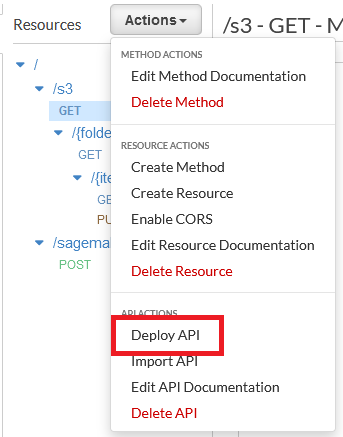
\includegraphics{pages/Chapter4/Chapter 4 Images/deploy_api_gateway.png}
    \caption{How to deploy API Gateway from within the API Gateway dashboard}
    \label{fig:deploy_api_gateway}
\end{figure}


\subsection{Pre-Processing Lambda}
For this section, the implementation of the pre-processing Lambda for the Laptop-To-Cloud pipeline follows a very similar implementation as described in \ref{fig:json_compression}. Where all 5 JSON files extracted from the .db file, must be uploaded into the Lambda function. The main differences being that now the JSON files have been uploaded into an S3 bucket from the laptop, so the cloud-based processing within Lambda is free to handle the processing. 

First the Lambda function must be setup to trigger on S3 create events (which include Put, Post, Update etc...). However, in order to ensure that all 5 JSON files are present before the processing begins, only .complete files are allowed to trigger the Lambda function, as stated in the design section for this pipeline, a .complete file is uploaded only after all 5 JSON files are uploaded.

This triggering on .complete file ensures all files will be available for the compression transformation. The compresson JSON file now sends the data to another S3 bucket (different from the source bucket), so as to avoid cluttering of the S3 bucket. The data can then be used for ML development or for classification as needed.


%Eu Jin's stuff
\subsection{Data Analysis, Pre-processing and Feature Extraction} 

Firstly, telemetry data set consisting of about 800 data points from 3 different devices with different MAC addressed are used in the JSON file format. The bucket containing this data is loaded into the JupyterLab IDE provided by the Sagemaker service.
 
From the telemetry data collected, data for the 5GHz-1 frequency will be investigated and analysed to be used to build the machine learning model. 
The JSON file containing the data is loaded into a data frame as shown in Figure \ref{fig_df}. The columns in the data frame displays the telemetry data parameters of each channel existing in the 2.4GHz, 5GHz-1 and 5GHz-2 bands.

\begin{figure}[ht]
    \centering
    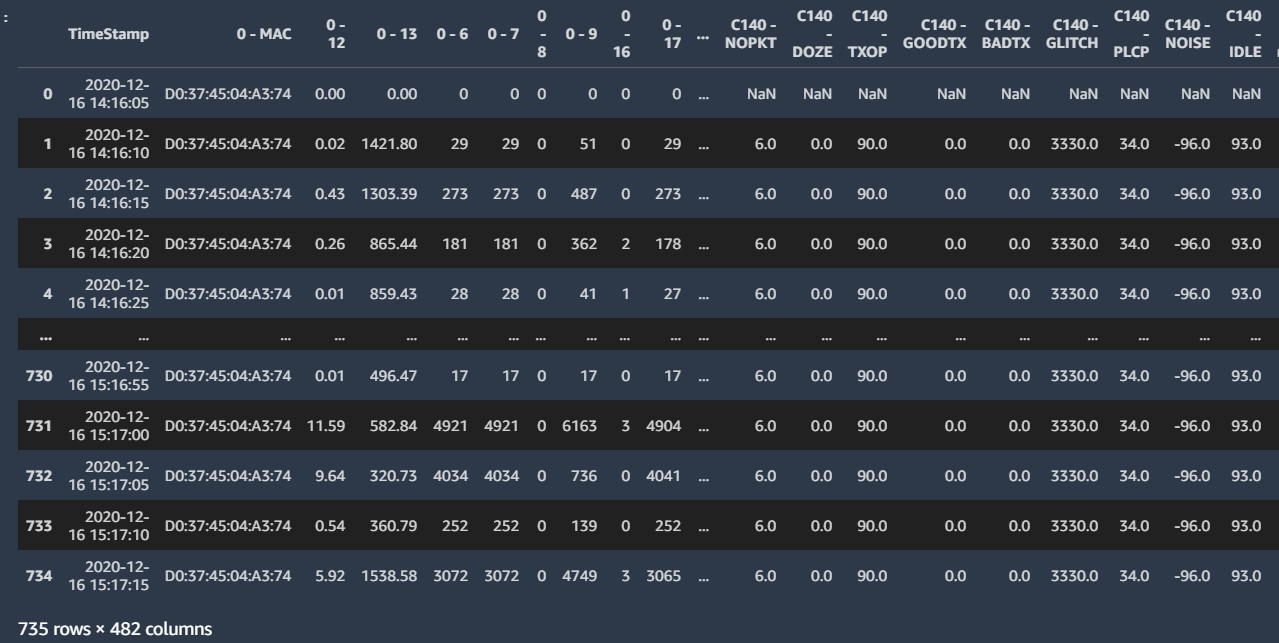
\includegraphics[scale=0.53]{pages/Chapter4/Chapter 4 Images/Dataframe.PNG}
    \caption{Data frame of JSON file.}
    \label{fig_df}
\end{figure}

There exists 8 channels under that particular frequency band which are channels 36, 40, 44, 48, 52, 56, 60 and 64. The parameters for channel 52 were filtered out and used as it is the most active and the other seven channels share the exact same data values. Missing values in the dataset were also removed to ensure uniformity. The data throughput rate for the three devices  respectively were then obtained for analysis shown in Figure \ref{fig_t3} and illustrated using a histogram. From observation of the data throughput rates, the device which is under the process of downloading a game shows the highest variation whereas there is little variation for the other two devices. Thus, the data throughput rate for the first device is filtered out to be used for further analysis. 

\begin{figure}[ht]
    \centering
    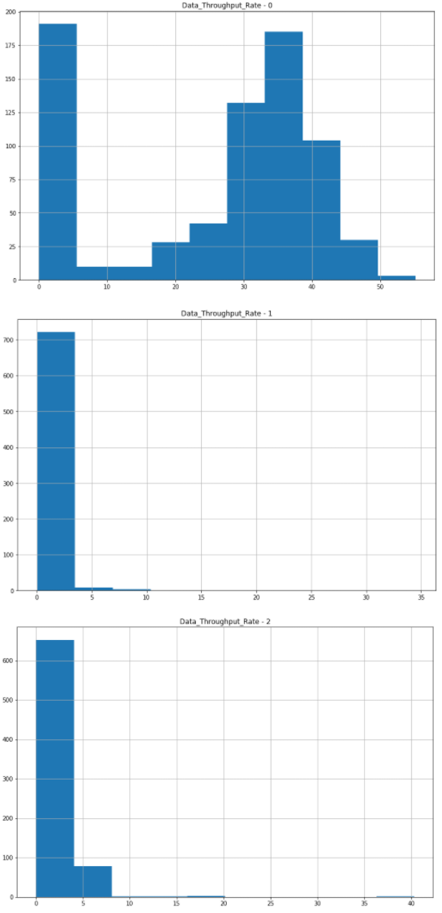
\includegraphics[scale=0.9]{pages/Chapter4/Chapter 4 Images/Throughput.PNG}
    \caption{Data Throughput rate for laptop, mobile phone and respectively}
    \label{fig_t3}
\end{figure}

Next, a heatmap for the correlation matrix which shows the relationship between the parameters of the telemetry data is obtained as shown in Figure \ref{fig_Cmatrix}. 

\begin{figure}[ht]
    \centering
    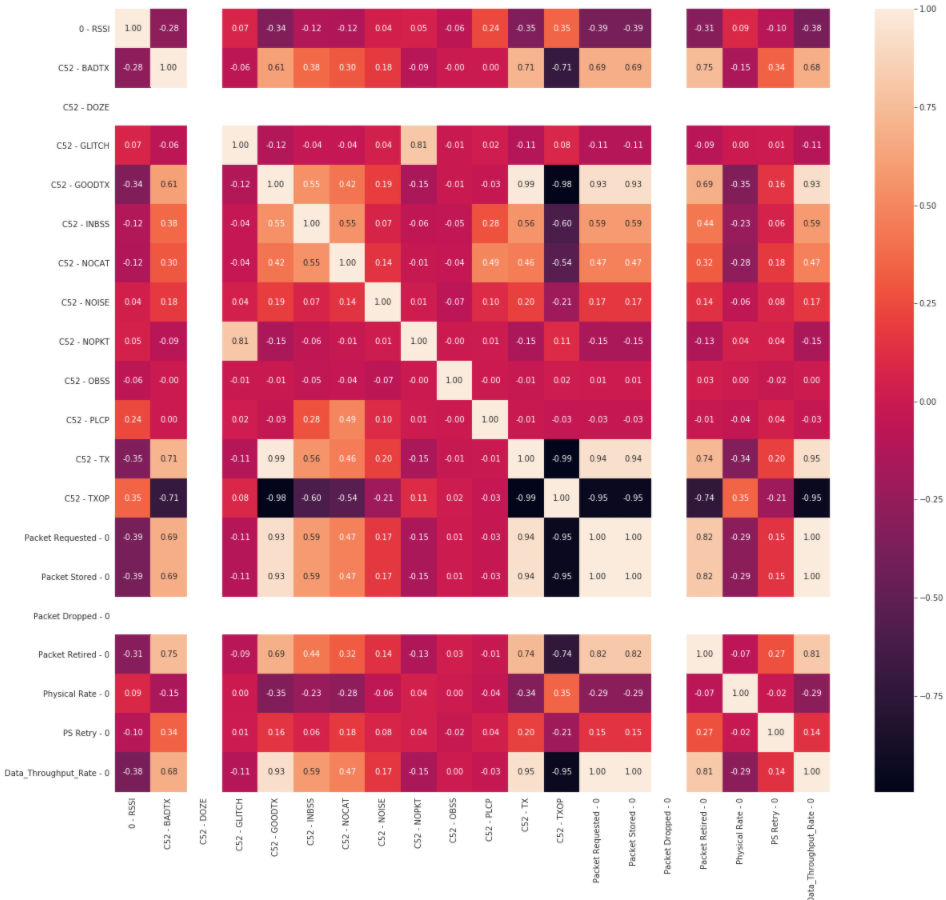
\includegraphics[width=14.5cm,height=15.2cm,keepaspectratio]{pages/Chapter4/Chapter 4 Images/Cmatrix.PNG}
    \caption{Heatmap Correlation Matrix}
    \label{fig_Cmatrix}
\end{figure}

The correlation coefficients were compared between each of the parameters with the data throughput rate. The coefficients were compiled and can be shown in table \ref{table:cc}. 

\begin{table}[ht]
\centering
\begin{center}
\begin{tabular}{ |c|c| } 
  \hline
 Parameters & Correlation coefficient , \textit{r}\\ 
  \hline\hline
 RSSI & -0.38\\ 
 BADTX & 0.68\\ 
 DOZE & -\\ 
 GLITCH & -0.11\\ 
 GOODTX & 0.93\\ 
 INBSS & 0.59\\ 
 NOCAT & 0.47\\ 
 NOISE & 0.17\\\ 
 NOPKT & -0.15\\ 
 OBSS & 0.00\\ 
 PLCP & -0.03\\ 
 TX & 0.95\\ 
 TXOP & -0.95\\ 
 Packet Requested & 1.0\\ 
 Packet Stored & 1.0\\  
 Packet Dropped & -\\ 
 Packet Retired & 0.81\\ 
 Physical Rate & -0.29\\  
 PS Retry & 0.14\\ 
 \hline
\end{tabular}
\caption{Correlation coefficients between the parameters and data throughput rate}
\label{table:cc}
\end{center}
\end{table}

The parameters with coefficient values with intervals of $0.6\leq r \leq 1$ and $-1\leq r \leq -0.6$ are chosen as the features that will be used to train and build the machine learning model. These parameters are chosen as they hold a strong correlation with the data throughput rate which ranges from a moderate to a very strong linear relationship. Therefore, the parameters that will be used as features are as follows: 

\begin{itemize}
    \item GoodTX
    \item BadTX
    \item TX
    \item TXOP
    \item Packet Requested
    \item Packet Stored
    \item Packet Retired
\end{itemize}
 
Bar plots are obtained to show a better illustration of the relationship between the selected parameters on the y-axis and data throughput rate on the x-axis. The relationship between the packet requested, packet stored and packet retired with throughput is shown in Figure \ref{fig_bp1}. From the plot, it can be seen that the three parameters increases with data throughput rate.
Finally, the relationship between the BadTX and TXOP parameters with throughput rate is shown in Figure \ref{fig_bp3}.
\begin{figure} [ht]
    \centering
    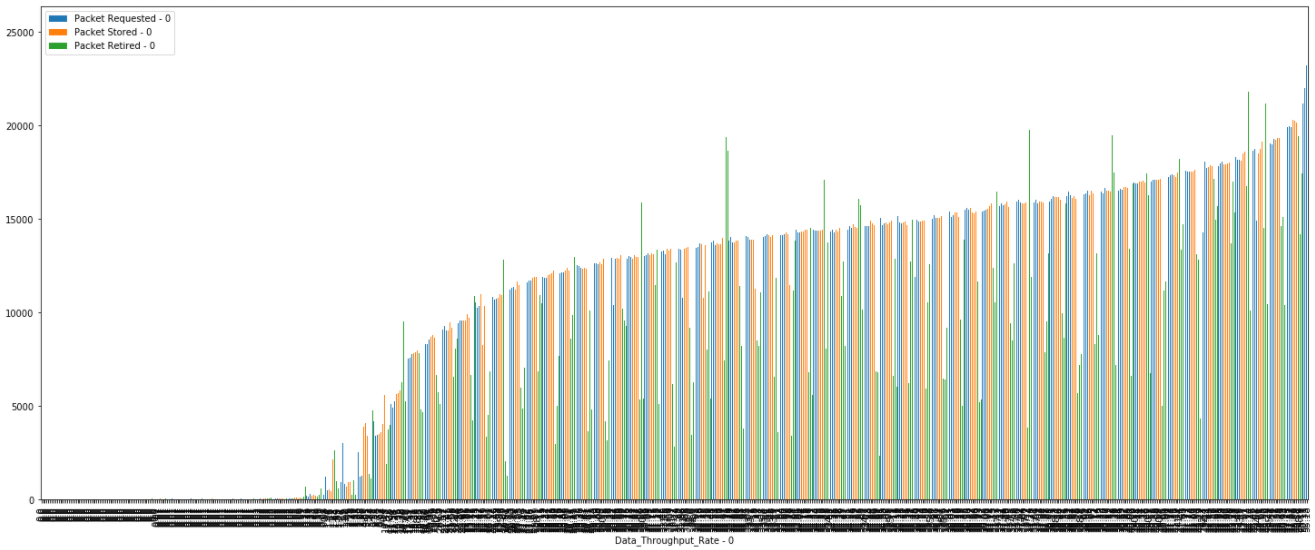
\includegraphics[scale = 0.52]{pages/Chapter4/Chapter 4 Images/Bplot1.PNG}
    \caption{Barplot of Packet Requested, Stored and Retired against Data Throughput Rate}
    \label{fig_bp1}
\end{figure}

Next, the relationship between the TX and GoodTX parameters with throughput rate is shown in Figure \ref{fig_bp2}. When the two parameters increase in value, the data throughput rate also increases.
\begin{figure} [ht]
    \centering
    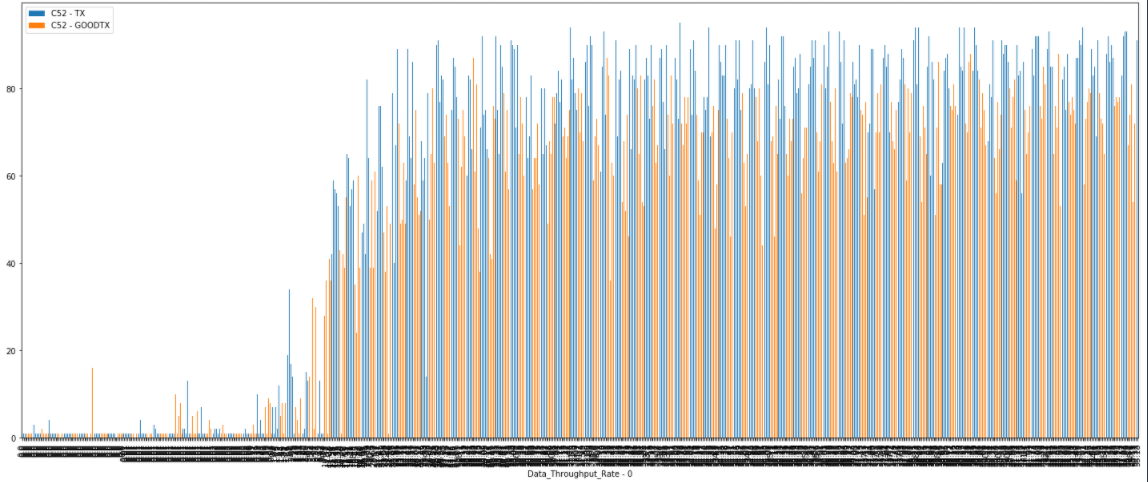
\includegraphics[width=14.6cm,height=200.0cm,keepaspectratio]{pages/Chapter4/Chapter 4 Images/Bplot2.PNG}
    \caption{Barplot of GOODTX and TX against Data Throughput Rate}
    \label{fig_bp2}
\end{figure}

Finally, the relationship between the BadTX and TXOP parameters with throughput rate is shown in Figure \ref{fig_bp3}. From the barplot obtained, the TXOP parameter decreases when the data throughput rate increases. On the other hand, the BadTX increases at a slow rate as the data throughput rate increases.
\begin{figure} [ht]
    \centering
    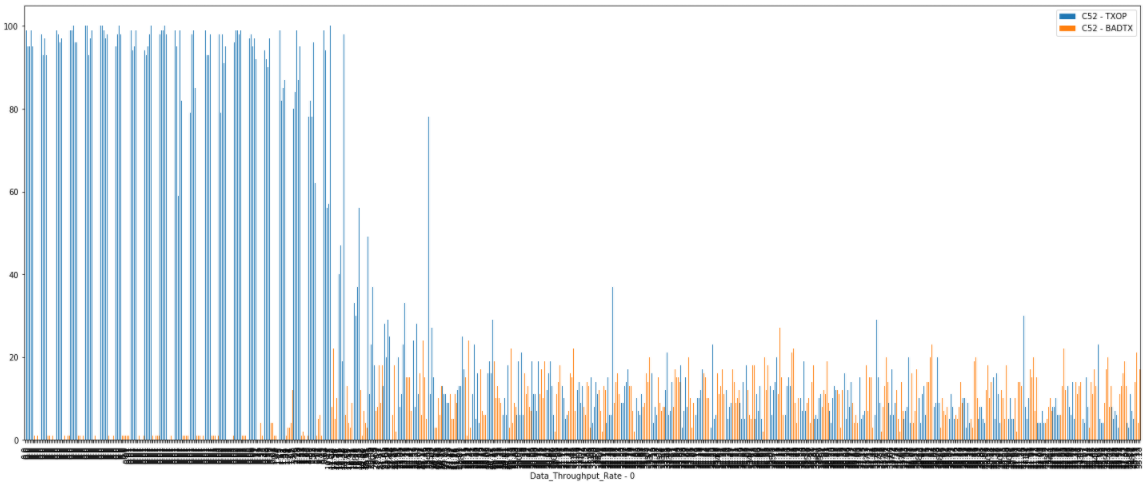
\includegraphics[width=14.6cm,height=200.0cm,keepaspectratio]{pages/Chapter4/Chapter 4 Images/Bplot3.PNG}
    \caption{Barplot of BADTX and TXOP against Data Throughput Rate}
    \label{fig_bp3}
\end{figure}

After this analysis,the creation of the target variable (class) known as data throughput strength based on data throughput rate intervals was implemented and can be shown in table. \ref{table:class}. Five different classes are created: \textbf{Very Weak}, \textbf{Weak}, \textbf{Moderate}, \textbf{Strong} and \textbf{Very Strong}.

\begin{table}[ht]
\centering
\begin{center}
\begin{tabular}{ |c|c| } 
 \hline
 Data Throughput Rate/Mbps & Data Throughput Strength\\ 
  \hline\hline
 0-9 & Very Weak\\ 
 10-19 & Weak\\ 
 20-29 & Moderate \\ 
 30-39 & Strong\\ 
 40 and above & Very Strong\\ 

 \hline
\end{tabular}
\caption{Data Throughput Strength Class implementation based on Data Throughput Rate with 800 Data Points}
\label{table:class}
\end{center}
\end{table}

The seaborn library imported as \textit{sns}, is used to produce a pairplot which shows the distribution between two features in different classes of data throughput strength implemented as shown in Figure \ref{fig_pp}. It also shows the distribution of each feature in the five different classes.

\begin{figure} [ht]
    \centering
    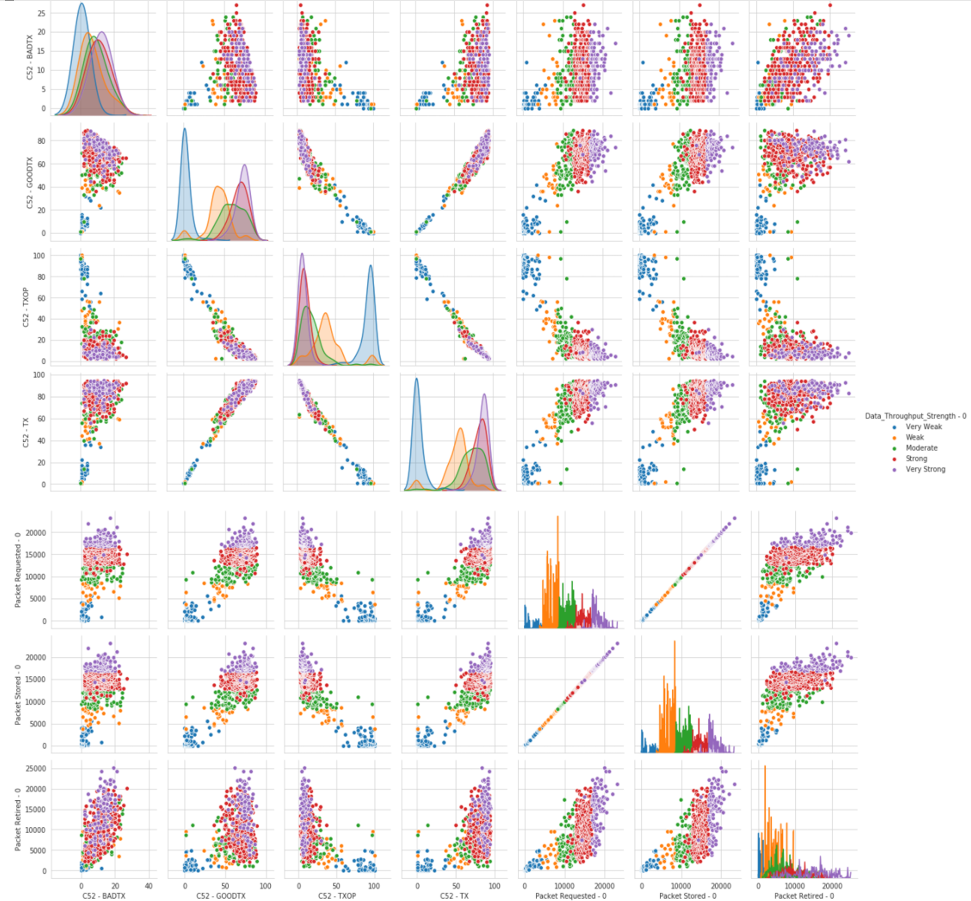
\includegraphics[width=14.6cm,height=200.0cm,keepaspectratio]{pages/Chapter4/Chapter 4 Images/Pairplot.PNG}
    \caption{SNS Pairplot}
    \label{fig_pp}
\end{figure}
 
 From the testing phase in \ref{Section: Testing Phase of ML Model}, the model has an accuracy of 89\% even though it has a high accuracy during the validation phase. This problem occurs because there is too little data and causes overfitting even with the hyperparameters tuned. Thus, a data set containing approximately 6000 data points is collected. The data is preprocessed where the data throughput rate interval for each class were adjusted to accommodate higher rates. The updated interval for each data throughput strength class is shown in Table. \ref{table:class2}.
 
\begin{table}[ht]
\centering
\begin{center}
\begin{tabular}{ |c|c| } 
 \hline
 Data Throughput Rate/Mbps & Data Throughput Strength\\ 
  \hline\hline
0-9 & Very Weak\\ 
10-29 & Weak\\ 
30-49 & Moderate \\ 
50-99 & Strong\\ 
100 and above & Very Strong\\ 

 \hline
\end{tabular}
\caption{Data Throughput Strength Class implementation based on Data Throughput Rate with 6000 Data Points}
\label{table:class2}
\end{center}
\end{table}
 
\subsection{Training and Validation of Machine Learning Model} 
The features are then normalized and prepared to be used to train and build the machine learning model. A clearer workflow of the implementation of training, validating and testing the model is shown in Figure \ref{fig_mlmodel}.

\begin{figure} [ht]
    \centering
    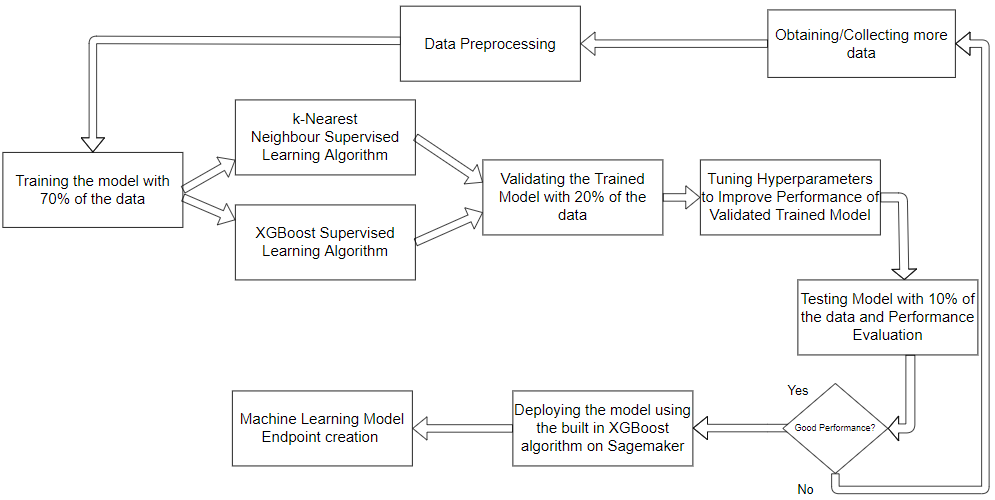
\includegraphics[scale = 0.69]{pages/Chapter4/Chapter 4 Images/Work Flow.PNG}
    \caption{Detailed Block Level Diagram of Machine Learning Model Development}
    \label{fig_mlmodel}
\end{figure}

The dataset is split into a ratio of 70:20:10. 70\% of the data is used to train the model, 20\% of the data is used to validate the model and the remaining 10\% is used to test and evaluate the performance of the final machine learning model. 

\subsubsection{k-Nearest Neighbour Algorithm with Scikit-Learn}
The k-Nearest Neighbour supervised learning algorithm is used to build the model within Sagemaker without deployment. The model is validated with the validation set after it is being trained. Several hyperparameters are tuned such as the number of neighbours, \textit{k} and the distance function to improve the performance of the trained model. The value of k is varied from 1 to 10 with two different distance functions which are the Euclidean and Manhattan functions. The performance of the trained model using the validation set is measured with the accuracy metric. The results are transferred into a table shown in Table \ref{table:euclidean} and Table \ref{table:manhattan} respectively.

\begin{table}[ht]
\centering
\begin{center}
\begin{tabular}{ |c|c| } 
  \hline
 The number of neighbors, k  & Accuracy/\%\\ 
  \hline\hline
1 & 95.9\\ 
2 & 96.6\\ 
3 & 95.9\\ 
4 & 98.6\\ 
5 & 96.6\\ 
6 & 95.9\\ 
7 & 97.3\\ 
8 & 96.6\\\ 
9 & 97.3\\ 
10 & 95.9\\ 
\hline
\end{tabular}
\caption{Accuracy of validated trained model using the Euclidean distance function }
\label{table:euclidean}
\end{center}
\end{table}

\begin{table}[ht]
\centering
\begin{center}
\begin{tabular}{ |c|c| } 
  \hline
 The number of neighbors, k  & Accuracy/\%\\ 
  \hline\hline
1 & 95.2\\ 
2 & 98.6\\ 
3 & 97.3\\ 
4 & 98.6\\ 
5 & 97.3\\ 
6 & 97.3\\ 
7 & 97.9\\ 
8 & 97.9\\\ 
9 & 97.3\\ 
10 & 96.6\\ 

 \hline
\end{tabular}
\caption{Accuracy of validated trained model using the Manhattan distance function}
\label{table:manhattan}
\end{center}
\end{table}
 
From the validation results with the Euclidean distance function , the \textit{k} value of 4 gives the best performance with an accuracy of 98.6\%. For the results with the Manhattan distance function, a \textit{k} value of also gives the same accuracy of about 98.6\%. Therefore, both distance functions with a \textit{k} value of 4 can be used to train the model and evaluate the model performance with the test data.


Next, the model is retrained with the k-Nearest Neighbour algorithm using the 6000 data points collected. The hyperparameters were maintained and used in the training and validating phases. The results of the trained model with the validation set is recorded in Table \ref{table:euclidean2} and Table \ref{table:manhattan2} respectively.
\begin{table}[ht]
\centering
\begin{center}
\begin{tabular}{ |c|c| } 
  \hline
 The number of neighbors, k  & Accuracy/\%\\ 
  \hline\hline
1 & 97.8\\ 
2 & 97.4\\ 
3 & 98.2\\ 
4 & 98.2\\ 
5 & 98.3\\ 
6 & 98.4\\ 
7 & 98.6\\ 
8 & 98.5\\ 
9 & 98.6\\ 
10 & 98.3\\ 
\hline
\end{tabular}
\caption{Accuracy of validated trained model using the Euclidean distance function }
\label{table:euclidean2}
\end{center}
\end{table}

\begin{table}[ht]
\centering
\begin{center}
\begin{tabular}{ |c|c| } 
  \hline
 The number of neighbors, k  & Accuracy/\%\\ 
  \hline\hline
1 & 97.8\\ 
2 & 97.5\\ 
3 & 98.2\\ 
4 & 98.1\\ 
5 & 98.3\\ 
6 & 98.3\\ 
7 & 98.6\\ 
8 & 98.5\\\ 
9 & 98.4\\ 
10 & 98.3\\ 

 \hline
\end{tabular}
\caption{Accuracy of validated trained model using the Manhattan distance function}
\label{table:manhattan2}
\end{center}
\end{table}

\subsubsection{XGBoost Algorithm with Sagemaker Python SDK}
\label{xgboost-training}
Next, the built-in XGBoost supervised learning algorithm within Sagemaker is used to train and deploy the model. There are several steps required to prepare the data before training the model with the Sagemaker Python SDK. Firstly, the class of each data point has to be encoded with numeric values. The numeric values which represents each class is shown in Table \ref{table:class}. 
The column containing the class (target variable) has to be moved to the first column in the dataframe with its name removed. The dataset is then converted and stored as a CSV file. The XGBoost algorithm version 1.2-1 is used for the model training. The hyperparameters used are shown in table \ref{table:xg}. The training process can be shown in Figure \ref{fig_train}.

\begin{figure} [ht]
    \centering
    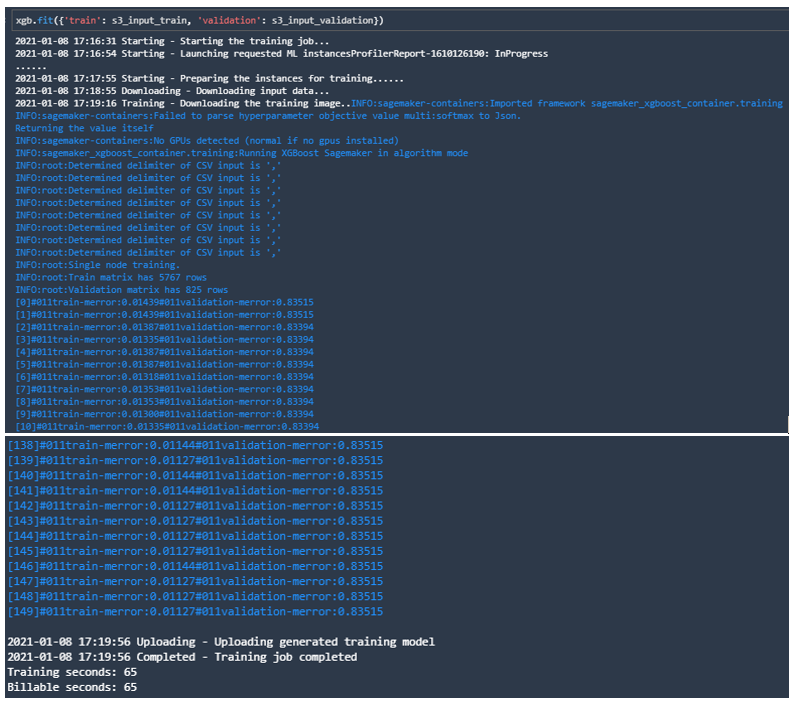
\includegraphics[scale = 0.8]{pages/Chapter4/Chapter 4 Images/Training.PNG}
    \caption{Snippet of Training the Machine Learning Model in Sagemaker}
    \label{fig_train}
\end{figure}

After the model is trained with this algorithm, it will then be deployed with an endpoint being created. A variable will be created for the deployed trained model. This variable can then be used to validate the trained model using the validation data set. The accuracy of obtained for the validated trained model is about 28.4\% for the dataset containing approximately 800 data points. The hyperparameters were adjusted and still returns a low accuracy classifier.
On the other hand, the accuracy obtained for the validated trained model is about 98.8\% for the dataset containing approximately 6000 data points.

\begin{table}[ht]
\centering
\begin{center}
\begin{tabular}{ |c|c| } 
  \hline
 Class  & Numeric Value\\ 
  \hline\hline
Moderate & 0\\ 
Strong & 1\\ 
Very Strong & 2\\ 
Very Weak & 3\\ 
Weak & 4\\ 

 \hline
\end{tabular}
\caption{Numeric Representation for Each Class}
\label{table:class}
\end{center}
\end{table}

\begin{table}[ht]
\centering
\begin{center}
\begin{tabular}{ |c|c| } 
  \hline
Hyperparameters  & Values\\ 
  \hline\hline
Max depth & 4\\ 
Learning rate (eta) & 0.2\\ 
Gamma & 4\\ 
Subsample & 0.5\\ 
Number of rounds & 150\\ 


 \hline
\end{tabular}
\caption{Hyperparameters for XGBoost Model}
\label{table:xg}
\end{center}
\end{table}

\subsection{Deploying Sagemaker Endpoint} 
When the machine learning model is deployed, an endpoint will be created during the process which can be shown in Figure \ref{fig_endpoint}. For example, the endpoint created for the deployed model has a name called ``sagemaker-xgboost-2020-12-22-20-52-53-943''. 

\begin{figure} [ht]
    \centering
    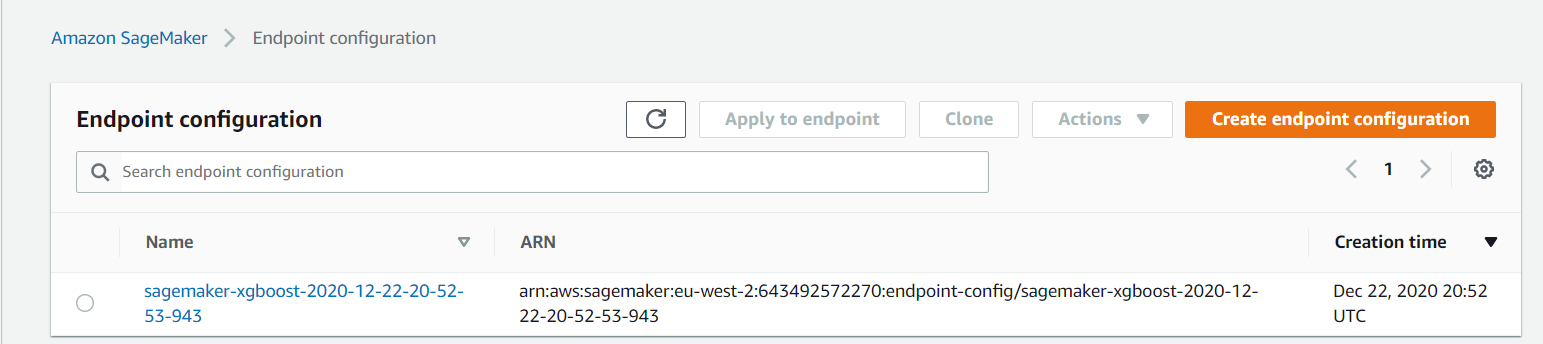
\includegraphics[scale= 0.44]{pages/Chapter4/Chapter 4 Images/Endpoint.PNG}
    \caption{Endpoint Creation}
    \label{fig_endpoint}
\end{figure}

This endpoint of the trained model can be invoked using Amazon API Gateway and AWS Lambda where it can be used to predict or classify data. A Lambda function is first created to call the Sagemaker runtime invoke endpoint. During this stage, the policy of the IAM execution role is edited such that it gives permission to the Lambda function to invoke the model endpoint which can be shown in Figure \ref{fig_policy}. 

\begin{figure} [ht]
    \centering
    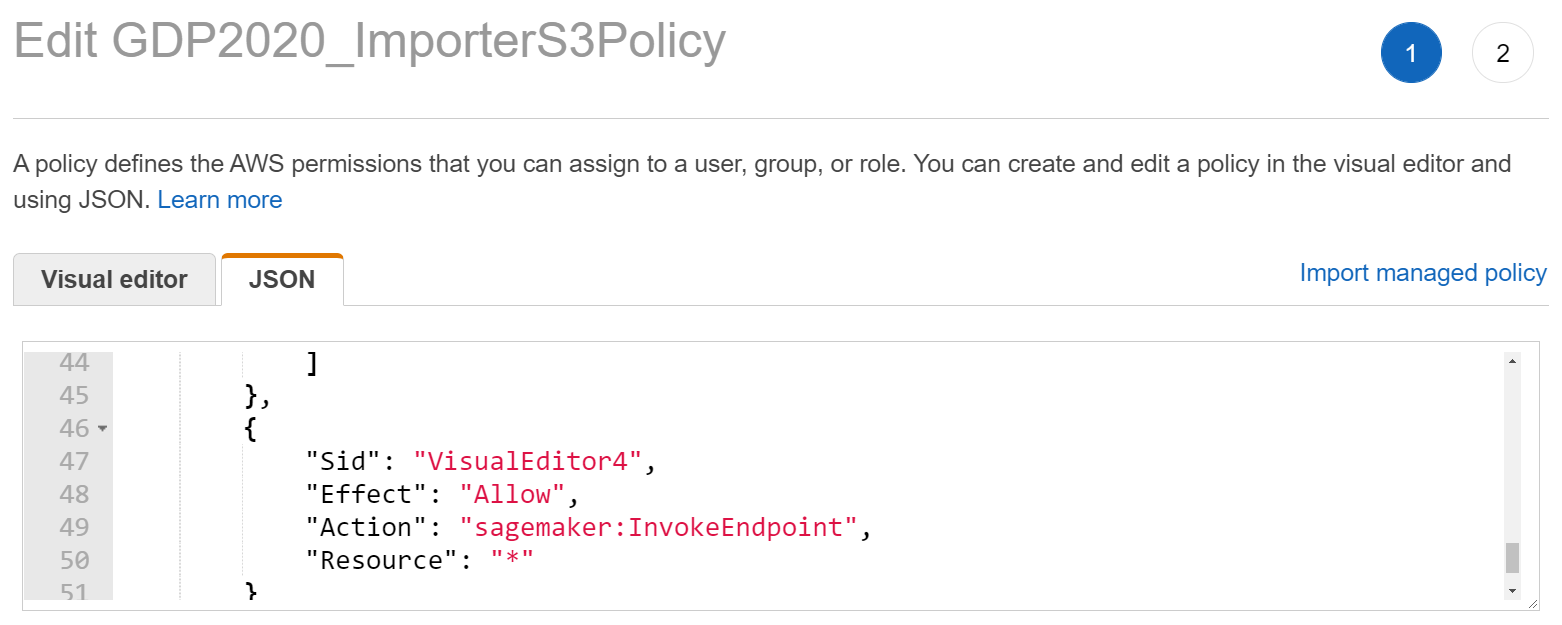
\includegraphics[scale =0.43]{pages/Chapter4/Chapter 4 Images/Policy.PNG}
    \caption{Policy Added for Endpoint Permission Access by the Lambda Function}
    \label{fig_policy}
\end{figure}

Next, the endpoint name is included in the environment variable for the Lambda function which will be made available to the code for the invocation request. This step can be shown in Figure \ref{fig_env}. 

\begin{figure} [ht]
    \centering
    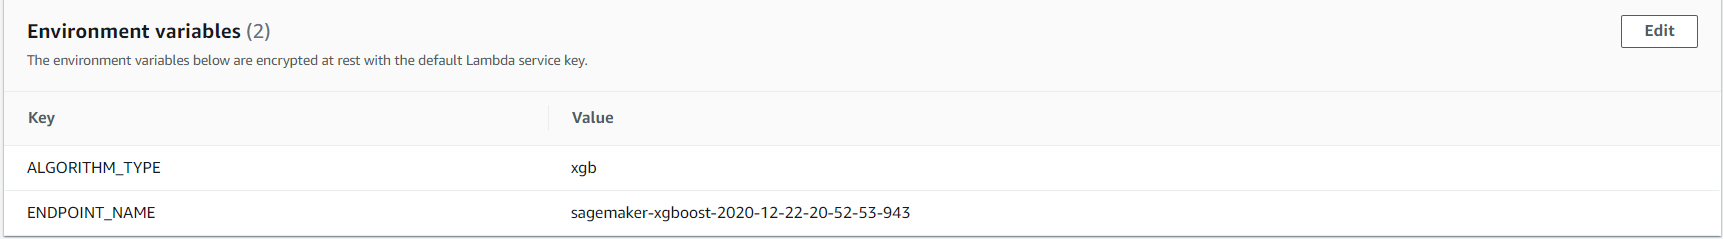
\includegraphics[width=14.0cm,height=2.5cm,scale =0.45]{pages/Chapter4/Chapter 4 Images/ENVIRON.PNG}
    \caption{Environmental Variable}
    \label{fig_env}
\end{figure}

Moving on forward, an API Gateway is created where it triggers an event that invokes the Lambda function. The event triggered would be the test data passing through it. The final setup of the API Gateway is shown in Figure \ref{fig_api}. An invoke URL will be obtained when the API Gateway is deployed. 

\begin{figure} [ht]
    \centering
    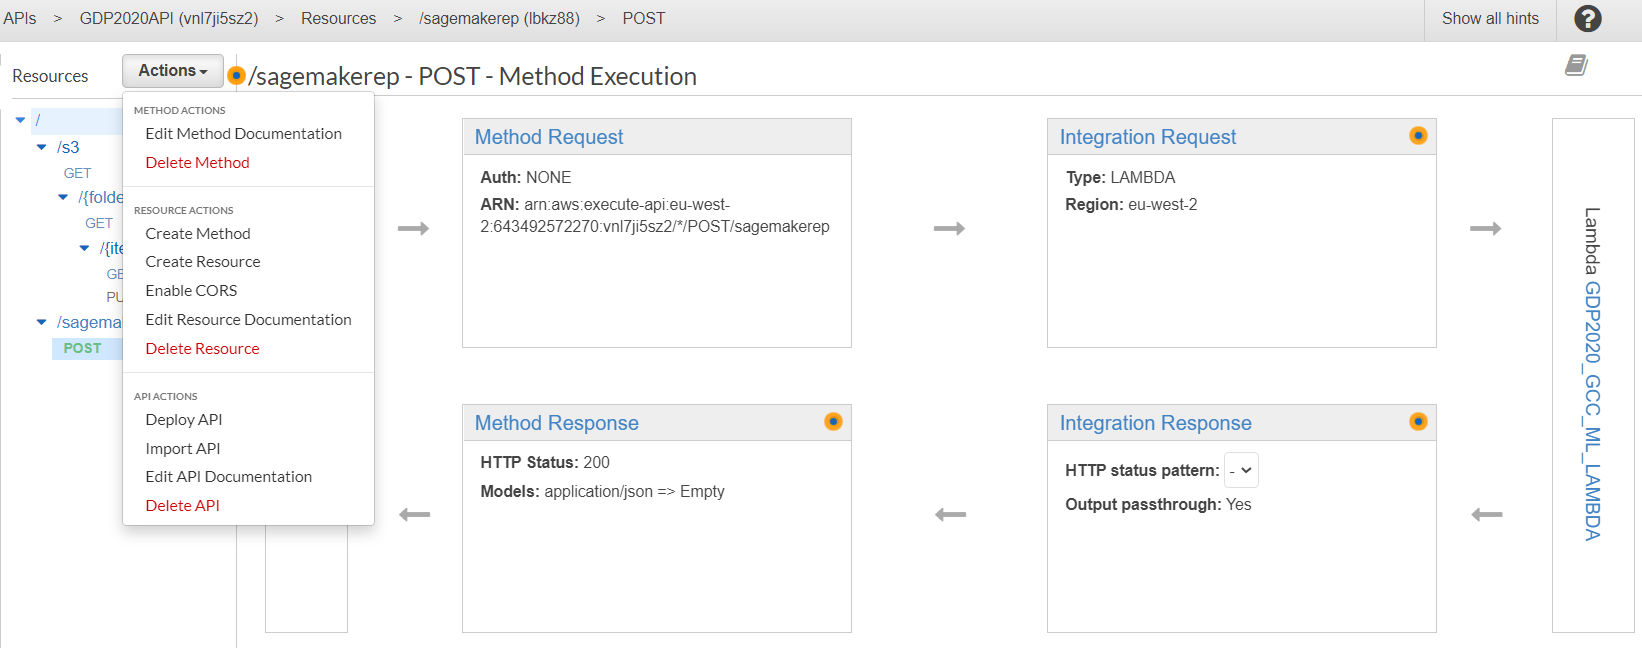
\includegraphics[width=14.6cm,height=200.0cm,keepaspectratio]{pages/Chapter4/Chapter 4 Images/API Gateway.PNG}
    \caption{API Gateway setup for Lambda function to Invoke Endpoint}
    \label{fig_api}
\end{figure}


  
% \section{Machine Learning Model Deployment}